% ==============================================================================
% 第 14 章：处处皆相似 (Similarities Everywhere)
% ==============================================================================

\chapter{处处皆相似}
\label{sec:ch14_similarities}

如果你完成了第二部分中的（部分）练习，你会发现许多解法看起来惊人地相似。事实上，这种相似性可能会诱使你复制一个问题的解决方案，直接作为下一个问题的解答。但\term{切莫复制代码}，哪怕是你自己写的代码也不行。相反，你必须对相似的代码片段进行\term{抽象}（abstract）。本章将系统地教你如何进行抽象。

我们消除相似性的手段是特定于\term{中级学生语言}（Intermediate Student Language，简称 \term{ISL}）的。几乎所有其他主流编程语言都提供了类似的机制；在面向对象语言中，你还会发现额外的抽象机制。无论如何，这些机制都具有本章所阐述的基本特征，因此这里讲解的设计理念同样适用于其他各种计算语境。

\begin{notebox}[切换教学语言]
在 DrRacket 中，请从菜单栏的“Language”（语言）菜单中，选择“How to Design Programs”子菜单下的“Intermediate Student”（中级学生语言）。
\end{notebox}

% ------------------------------------------------------------------------------
\section{函数中的相似性}
\label{sec:14_1}

设计配方决定了函数的基本组织形式，因为模板是直接从数据定义中提炼出来的，完全不依赖于函数的具体目的。因此，处理同一种数据的函数看起来彼此相似也就不足为奇了。

请观察图~\ref{fig:86} 中的两个函数，它们都接收一个字符串列表并查找特定的字符串。左边的函数查找 \code{"dog"}，右边的函数查找 \code{"cat"}。这两个函数几乎毫无二致：每个函数都以字符串列表作为输入；每个函数体都由一个包含两个分支的 \code{cond} 表达式构成；当输入为空列表 \code{'()} 时，都产生 \code{\#false}；每个函数都使用 \code{or} 表达式来判断列表的首项是否为目标项，如果不是，则通过递归在列表的剩余部分中继续查找。唯一的区别在于嵌套表达式中用于比较的具体字符串：\code{contains-dog?} 使用了 \code{"dog"}，而 \code{contains-cat?} 使用了 \code{"cat"}。为了突出这些差异，图中对这两个字符串进行了阴影高亮。

\begin{figure}[htbp]
  \centering
  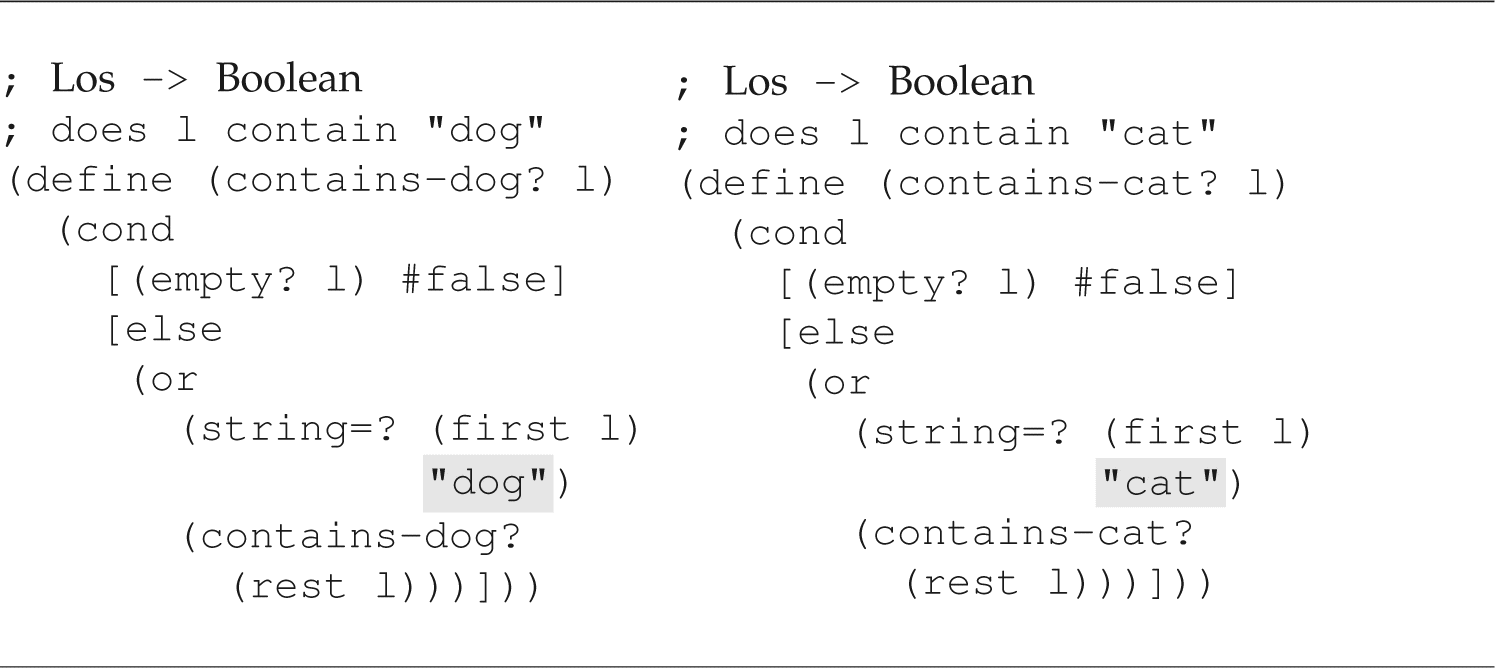
\includegraphics[width=0.85\textwidth]{images/00315.png}
  \caption{两个相似的函数}
  \label{fig:86}
\end{figure}

优秀的程序员往往“懒得”去定义好几个高度相近的函数。相反，他们会定义一个通用函数，既能在字符串列表中查找 \code{"dog"}，也能查找 \code{"cat"}。这个通用函数只需额外接收一项数据——即要查找的目标字符串——而在其他方面与原先的两个函数完全一致：

\begin{center}
  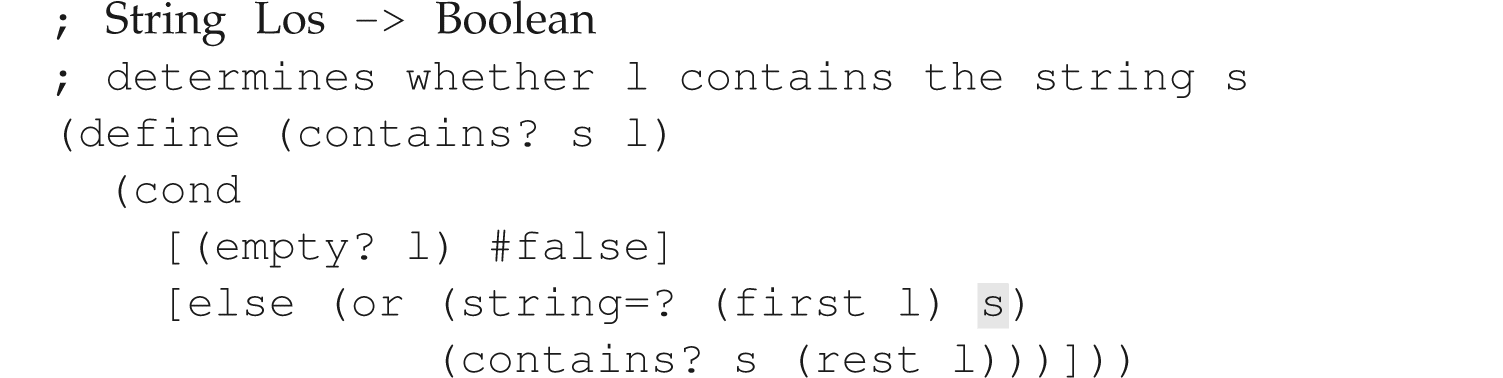
\includegraphics[width=0.85\textwidth]{images/00316.png}
\end{center}

如果你现在确实需要一个像 \code{contains-dog?} 这样的函数，只需将其定义为单行函数即可，对于 \code{contains-cat?} 也是如此。图~\ref{fig:87} 正是这么做的。你可以将它与图~\ref{fig:86} 进行简短对比，确保理解我们是如何从前者演进到后者的。最棒的是，有了 \code{contains?}，在字符串列表中查找任意字符串都变得轻而易举，我们再也不需要定义像 \code{contains-dog?} 这样专用的特殊函数了。

\begin{figure}[htbp]
  \centering
  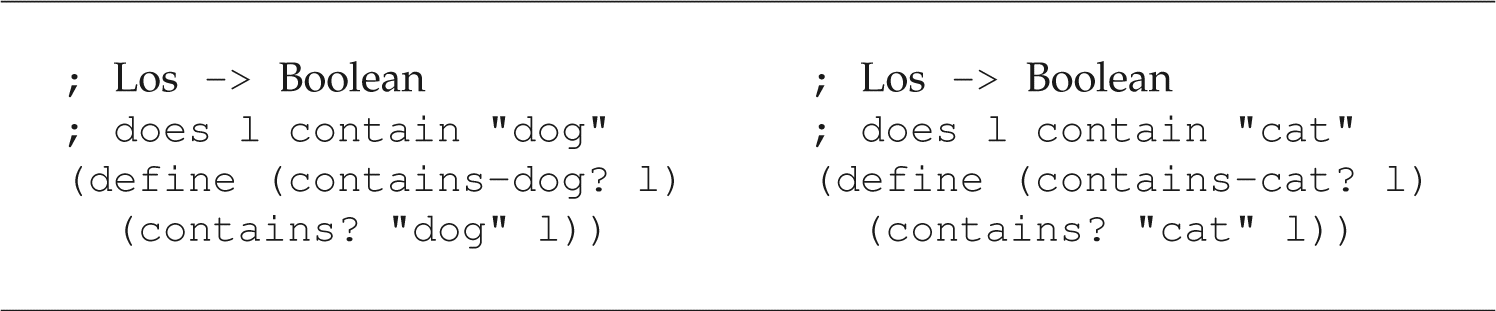
\includegraphics[width=0.85\textwidth]{images/00317.png}
  \caption{重新审视两个相似函数}
  \label{fig:87}
\end{figure}

你刚刚目睹的过程被称为\term{抽象}（abstraction），更准确地说，是\term{函数抽象}（functional abstraction）。对函数的不同版本进行抽象，是消除程序中重复与相似性的首要途径。正如你将看到的，消除相似性使得程序在长期维护中更容易保持稳健。

\begin{notebox}[“抽象”的数学来源]
计算机科学家从数学中借用了“抽象”这个术语。在数学中，“6”是一个抽象概念，因为它代表了对任意六个事物进行计数的所有方式。相比之下，“6 英寸”或“6 个鸡蛋”则是具体的使用形态。
\end{notebox}

\begin{exercise}{搜索单词}{235}
使用通用函数 \code{contains?}，分别定义在字符串列表中搜索 \code{"atom"}、\code{"basic"} 和 \code{"zoo"} 的函数。
\end{exercise}

\begin{exercise}{数字列表变换与抽象}{236}
为以下两个函数编写完整的测试套件：

\begin{center}
  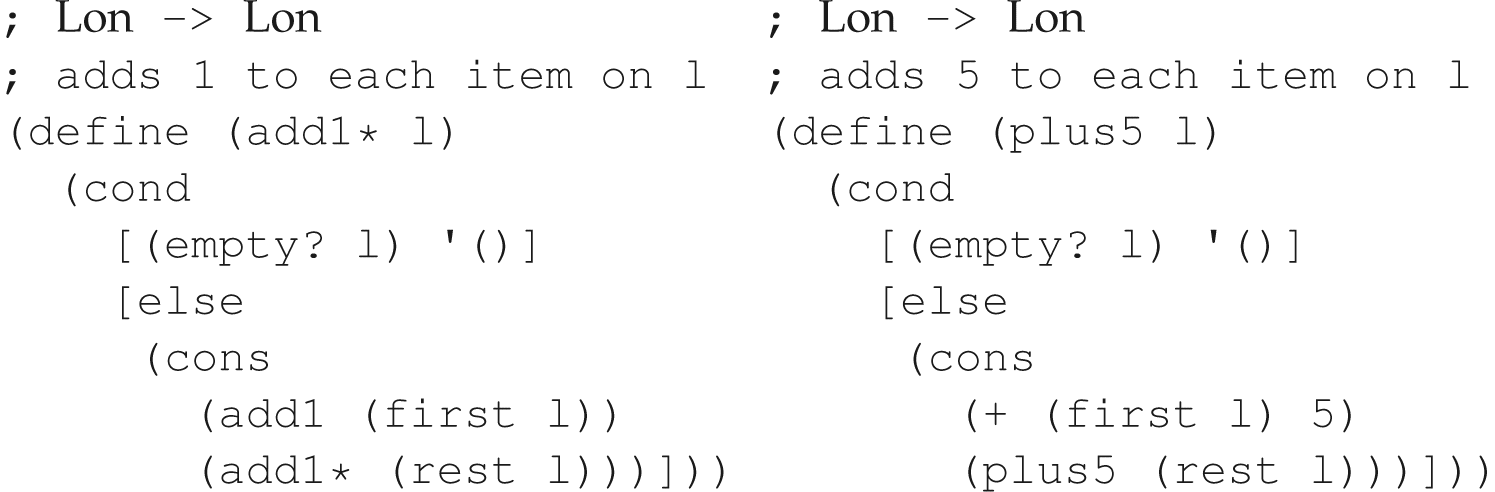
\includegraphics[width=0.85\textwidth]{images/00318.png}
\end{center}

然后对它们进行抽象。借助所提炼出的抽象函数，将上述两个函数重新定义为单行函数，并使用已有的测试套件确认修改后的定义能够正确工作。最后，再设计一个函数，从给定数字列表中的每个数字中减去 2。
\end{exercise}

% ------------------------------------------------------------------------------
\section{不同的相似性}
\label{sec:14_2}

在 \code{contains-dog?} 和 \code{contains-cat?} 的案例中，抽象看起来轻而易举。我们只需对比两个函数定义，用一个函数参数替换字面量字符串，并快速验证用抽象函数定义原函数十分容易即可。这种形式的抽象非常自然，以至于在本书的前两部分中已经多次自然而然地出现过。

本节将展示相同的原则如何衍生出一种更加强大的抽象形态。请看图~\ref{fig:88}。两个函数都接收一个数字列表和一个阈值。左边的函数产生列表中所有小于阈值的数字，而右边的函数则产生所有大于阈值的数字。

\begin{figure}[htbp]
  \centering
  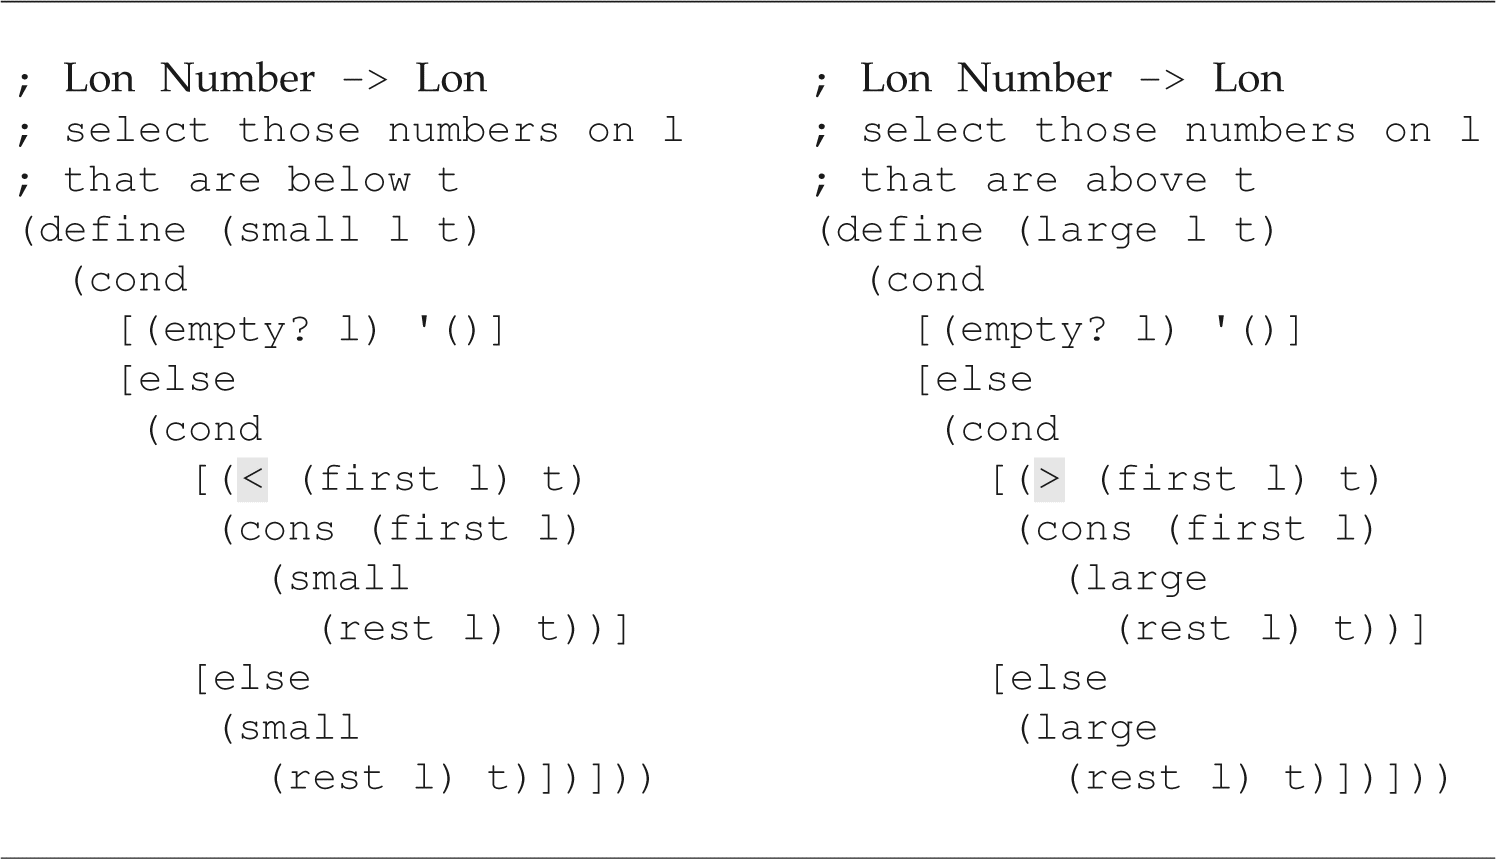
\includegraphics[width=0.85\textwidth]{images/00319.png}
  \caption{另外两个相似的函数}
  \label{fig:88}
\end{figure}

这两个函数仅在一处存在差异：用于决定列表中的数字是否应该包含在结果中的比较运算符。左边的函数使用了 \code{<}，右边的函数使用了 \code{>}。除此之外，除了函数名不同，两个函数在结构和逻辑上完全一模一样。

让我们遵循第一个示例的思路，引入一个额外的参数对这两个函数进行抽象。这一次，这个额外的参数所代表的不再是一个字符串，而是一个\term{比较运算符}：

\begin{center}
  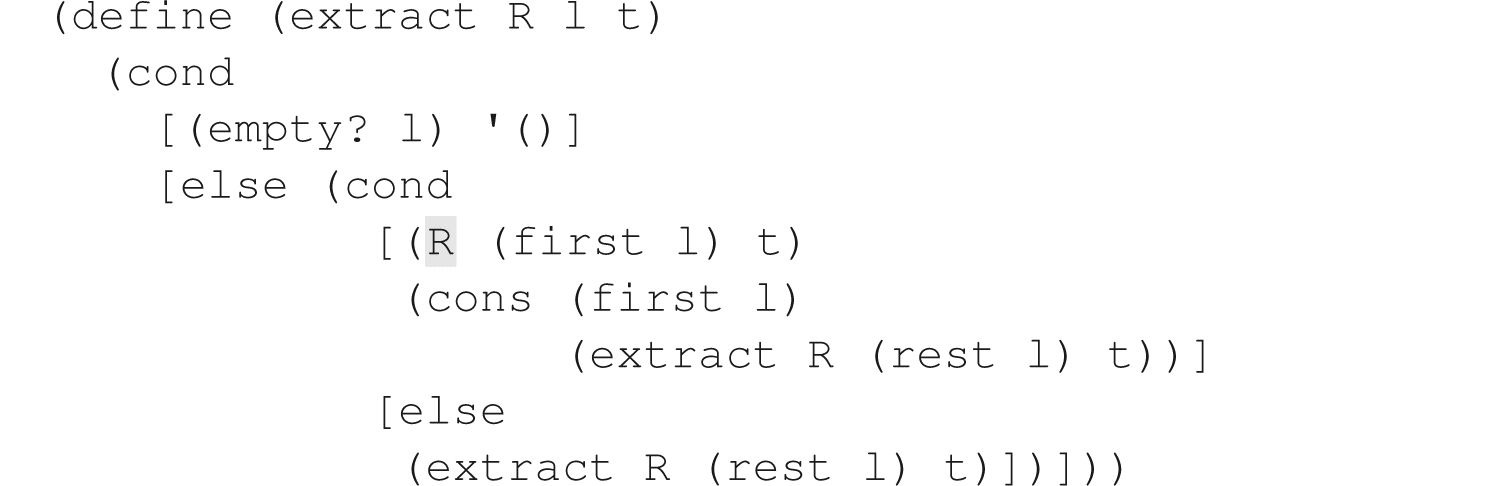
\includegraphics[width=0.85\textwidth]{images/00320.png}
\end{center}

要调用这个新函数，我们必须提供三个参数：一个比较两个数字的函数 \code{R}、一个数字列表 \code{l} 以及一个阈值 \code{t}。该函数随后会从 \code{l} 中提取出所有使得 \code{(R i t)} 求值为 \code{\#true} 的元素 \code{i}。

\begin{notebox}[驻足思考：函数作为参数！]
此时你应该停下来思考一下：这个定义真的合理吗？在没有任何多余仪式的情况下，我们竟然创建了一个\textbf{以函数作为参数的函数}——这可能是你以前从未见过的。然而事实证明，小巧简洁的教学语言 ISL 完全支持这类函数。而且，定义这种函数正是优秀程序员手中最强大的工具之一——即便在那些表面上似乎不直接支持高阶函数的语言中也是如此。
\end{notebox}

\begin{notebox}[微积分中的高阶函数]
如果你学过微积分，你一定遇到过微分算子和不定积分。它们本质上都是以函数作为输入并产生新函数的函数。不过，我们并不假设你学过微积分课程。
\end{notebox}

测试表明，\code{(extract < l t)} 的计算结果与 \code{(small l t)} 完全一致：

\begin{center}
  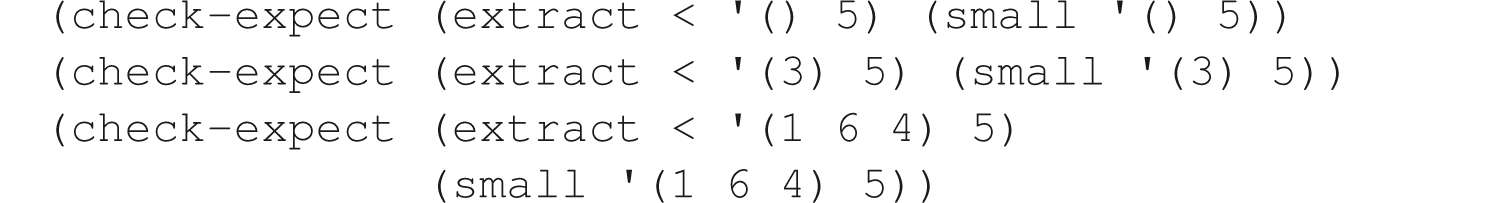
\includegraphics[width=0.85\textwidth]{images/00321.png}
\end{center}

类似地，\code{(extract > l t)} 产生与 \code{(large l t)} 相同的结果，这意味着你可以像这样重新定义原先的两个函数：

\begin{center}
  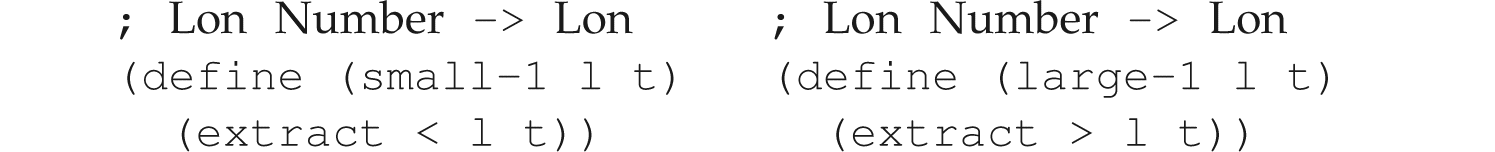
\includegraphics[width=0.85\textwidth]{images/00322.png}
\end{center}

这里最重要的领悟，并不仅仅在于 \code{small-1} 和 \code{large-1} 变成了单行定义。一旦拥有了像 \code{extract} 这样的抽象函数，你就可以将其广泛应用在其他场景中：

\begin{enumerate}
  \item \code{(extract = l t)}：提取出 \code{l} 中所有等于 \code{t} 的数字。
  \item \code{(extract <= l t)}：产生 \code{l} 中所有小于或等于 \code{t} 的数字列表。
  \item \code{(extract >= l t)}：计算出列表中所有大于或等于阈值的数字。
\end{enumerate}

事实上，传给 \code{extract} 的第一个参数根本不需要是 ISL 预定义的内置运算符。相反，你可以传入任何接收两个参数并返回布尔值的自定义函数。例如：

\begin{lstlisting}[language=BSL]
; Number Number -> Boolean
; 判断边长为 x 的正方形面积是否大于 c
(define (squared>? x c)
  (> (* x x) c))
\end{lstlisting}

也就是说，\code{squared>?} 检查命题 $x^2 > c$ 是否成立，它可以直接与 \code{extract} 配合使用：

\begin{lstlisting}[language=BSL]
(extract squared>? (list 3 4 5) 10)
\end{lstlisting}

这个调用将从 \code{(list 3 4 5)} 中提取出所有平方大于 10 的数字（即 4 和 5）。

\begin{exercise}{谓词求值}{237}
在 DrRacket 中求值 \code{(squared>? 3 10)} 与 \code{(squared>? 4 10)}。那么 \code{(squared>? 5 10)} 呢？
\end{exercise}

到目前为止，你已经看到抽象后的函数定义可以比原始函数有用得多。例如，\code{contains?} 比 \code{contains-dog?} 和 \code{contains-cat?} 更通用，而 \code{extract} 也比 \code{small} 和 \code{large} 更加强大。

抽象的另一个极其重要的优势在于：你现在为所有这些功能建立了\term{单点控制原则}（single point of control）。如果发现抽象函数中存在缺陷，只需修正其一处定义即可修复所有依赖于它的函数。同样，如果你找到了加速抽象函数计算或降低其能耗的优化方法，那么所有基于该函数定义的功能都将不费吹灰之力地享受到这些性能提升。接下来的练习将展示单点控制原则如何发挥效能。

\begin{notebox}[单点控制原则的普适价值]
抽象带来的这些好处存在于编程的各个层次：文字处理宏、电子表格公式、小型应用乃至大型工业级软件项目。为后者构建抽象正是驱动编程语言与软件工程前沿研究的核心动力。
\end{notebox}

\begin{exercise}{求最值函数的抽象与性能}{238}
将图~\ref{fig:89} 中的两个函数抽象为一个统一的通用函数。这两个函数都接收非空数字列表（Nelon）并返回一个数字。左边的函数求出列表中的最小值，右边的函数求出最大值。

\begin{center}
  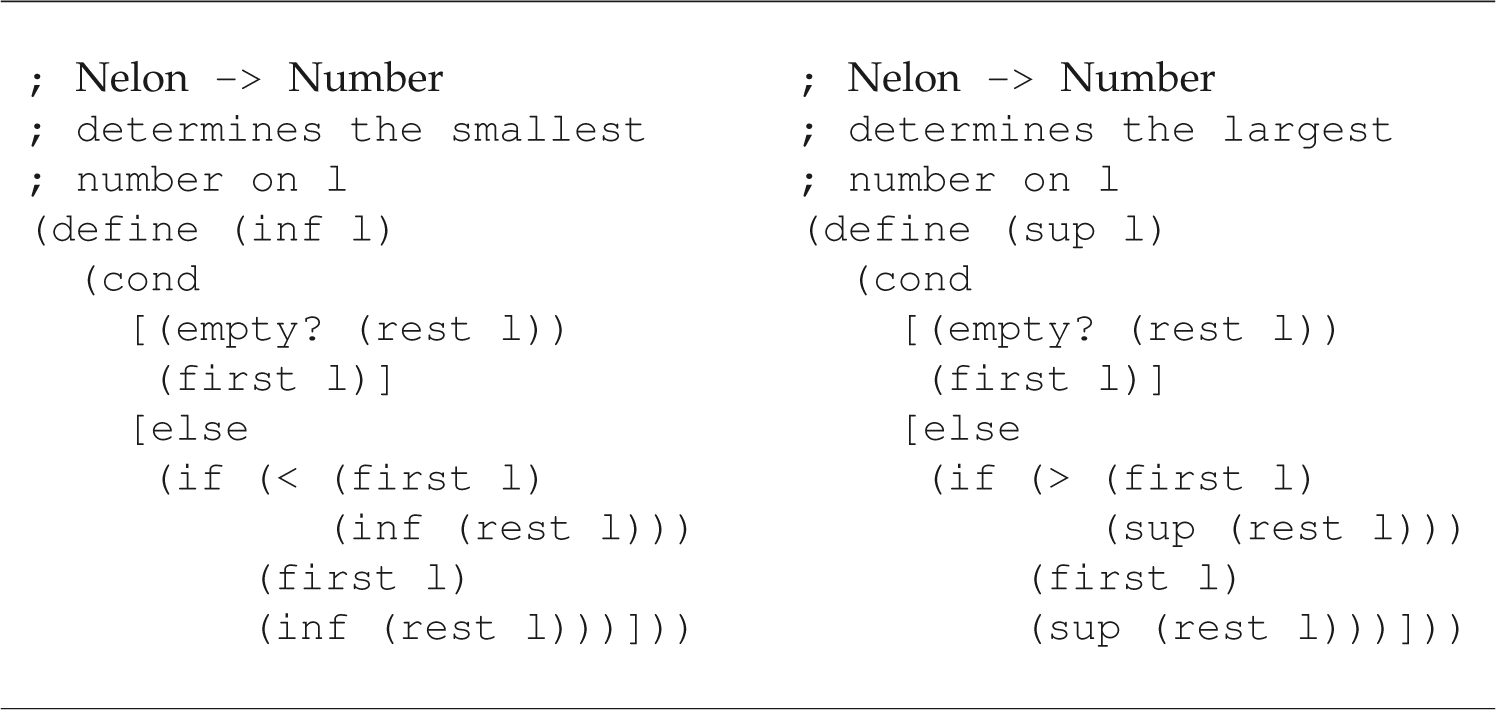
\includegraphics[width=0.85\textwidth]{images/00323.png}
  \captionof{figure}{在数字列表中查找下确界 (inf) 与上确界 (sup)}\label{fig:89}
\end{center}

借助该抽象函数定义 \code{inf-1} 与 \code{sup-1}。使用以下两个列表对它们进行测试：

\begin{center}
  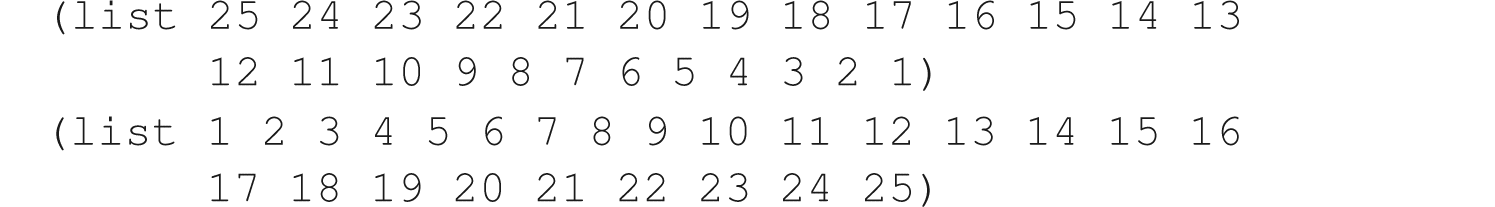
\includegraphics[width=0.85\textwidth]{images/00324.png}
\end{center}

为什么这些函数在处理某些长列表时会变得异常缓慢？

利用内置的 \code{max}（返回两个数中的较大者）和 \code{min}（返回较小者）重构原始函数。然后再次进行抽象，定义 \code{inf-2} 与 \code{sup-2}，并使用相同的测试输入重新测试。为什么这组新版本的运行速度会快得多？（关于此问题的另一种解答，请参见第 16.2 节）。
\end{exercise}

% ------------------------------------------------------------------------------
\section{数据定义中的相似性}
\label{sec:14_3}

现在请仔细观察以下两个数据定义：

\begin{center}
  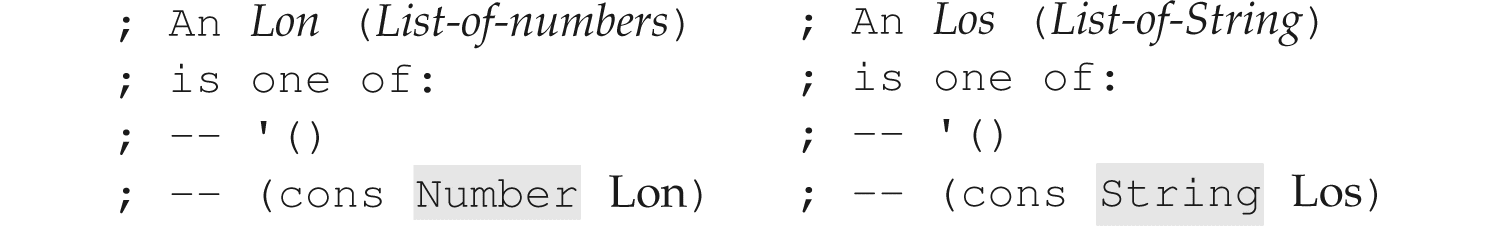
\includegraphics[width=0.85\textwidth]{images/00325.png}
\end{center}

左边定义了数字列表；右边描述了字符串列表。这两个数据定义极其相似。就像相似的函数一样，它们使用了两个不同的名称，但这无关紧要，因为换成任何名称都可以。唯一实质性的区别在于第二分支中 \code{cons} 内部的第一个位置，它规定了列表中包含哪种类型的元素。

为了消除这唯一的一处差异，我们把数据定义也当作函数来处理。我们引入一个参数，这使得数据定义看起来像一个函数；而在原先存在具体类型差异的地方，我们统一使用这个参数：

\begin{lstlisting}[language=BSL]
; A [List-of ITEM] is one of:
; -- '()
; -- (cons ITEM [List-of ITEM])
\end{lstlisting}

由于引入了参数，我们称这种抽象数据定义为\term{参数化数据定义}（parametric data definitions）。粗略地说，参数化数据定义抽象掉了对特定数据集合的直接引用，其方式与函数抽象掉特定具体值如出一辙。

核心问题当然是：这些参数的取值范围是什么？对于函数而言，形参代表一个未知的具体值；当函数被调用时，实参的具体值便确定下来。而对于参数化数据定义，形参代表\textbf{一整类值（数据集合）}。将某个数据集合的名称传递给参数化数据定义的过程被称为\term{实例化}（instantiation）。以下是抽象定义 \code{List-of} 的若干实例化示例：

\begin{itemize}
  \item 当我们写下 \code{[List-of Number]} 时，表示 \code{ITEM} 代表所有数字，因此它不过是 \code{List-of-numbers} 的另一个名字；
  \item 类似地，\code{[List-of String]} 与 \code{List-of-String} 定义了相同的数据类别；
  \item 如果我们定义了库存记录（Inventory Record）结构：
\begin{lstlisting}[language=BSL]
(define-struct ir [name price])
; An IR is a structure:
;   (make-ir String Number)
\end{lstlisting}
    那么 \code{[List-of IR]} 就是库存记录列表的类型名称。
\end{itemize}

按照惯例，我们在数据定义的形参中采用全大写字母（如 \code{ITEM}），而实参名称则按常规书写。

为了验证这些简写形式确实符合预期，我们可以用实际的数据定义名称（例如 \code{Number}）替换形参 \code{ITEM}，并为该数据定义赋予一个普通名称：

\begin{lstlisting}[language=BSL]
; A List-of-numbers-again is one of:
; -- '()
; -- (cons Number List-of-numbers-again)
\end{lstlisting}

由于数据定义是自引用的，我们替换了定义中的每一处参数。得到的结果与传统的数字列表定义完全相同，确实刻画了完全相同的数据类别。

让我们简要看看第二个例子，首先是一个结构体类型定义：

\begin{lstlisting}[language=BSL]
(define-struct point [hori veri])
\end{lstlisting}

以下是使用该结构体类型的两个不同数据定义：

\begin{center}
  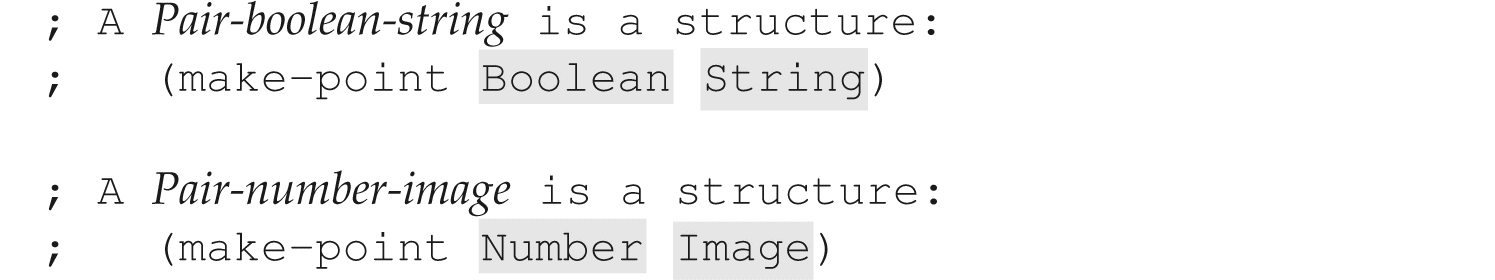
\includegraphics[width=0.85\textwidth]{images/00326.png}
\end{center}

在这种情况下，数据定义在两处存在差异（均以阴影标出）。\code{hori} 字段的差异彼此对应，\code{veri} 字段的差异亦是如此。因此，必须引入两个参数来构建抽象数据定义：

\begin{center}
  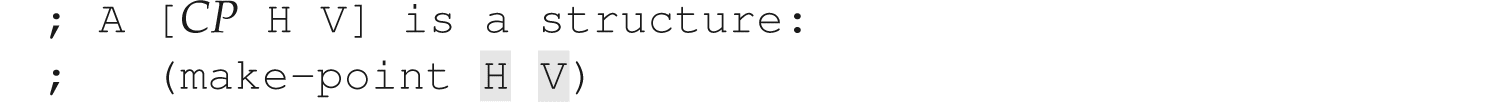
\includegraphics[width=0.85\textwidth]{images/00327.png}
\end{center}

这里 \code{H} 是用于 \code{hori} 字段数据集合的形参，而 \code{V} 则代表出现在 \code{veri} 字段中的数据集合。

要实例化一个带有两个参数的数据定义，你需要提供两个数据集合的名称。将 \code{Number} 和 \code{Image} 作为 \code{CP} 的参数，得到 \code{[CP Number Image]}，它描述了将数字与图像组合在一起的点；相比之下，\code{[CP Boolean String]} 则在点结构体中组合了布尔值与字符串。

\begin{exercise}{二元对的参数化数据定义}{239}
由两项构成的列表（二元对）是 ISL 编程中另一种频繁使用的数据形式。以下是带有两个参数的数据定义：

\begin{center}
  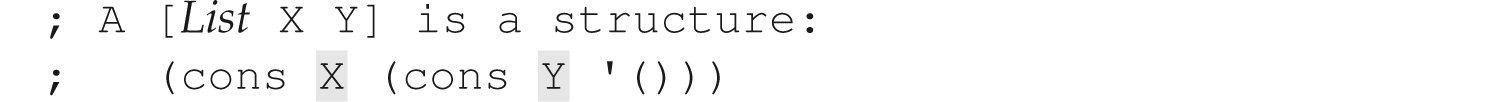
\includegraphics[width=0.85\textwidth]{images/00328.png}
\end{center}

实例化此定义以描述以下数据类别：
\begin{enumerate}
  \item 由两个 \code{Number} 构成的对；
  \item 由 \code{Number} 与 \code{1String} 构成的对；
  \item 由 \code{String} 与 \code{Boolean} 构成的对。
\end{enumerate}
并为这三种数据定义分别给出一个具体的实例。
\end{exercise}

一旦掌握了参数化数据定义，你就可以将它们组合嵌套使用，产生强大的表达效果。请看：

\begin{lstlisting}[language=BSL]
; [List-of [CP Boolean Image]]
\end{lstlisting}

最外层的标记是 \code{[List-of ...]}，这意味着你正在处理一个列表。至于列表中装的是什么样的数据，则需要观察其内部表达式：\code{[CP Boolean Image]} 将布尔值和图像组合在一个点中。因此，\code{[List-of [CP Boolean Image]]} 代表一个点列表，其中每个点都包含一个布尔值和一幅图像。类似地，\code{[CP Number [List-of Image]]} 则是 \code{CP} 的一种实例化，它将一个数字与一个图像列表组合在一起。

\begin{exercise}{嵌套结构的参数化抽象}{240}
以下是两个奇特但极其相似的数据定义：

\begin{center}
  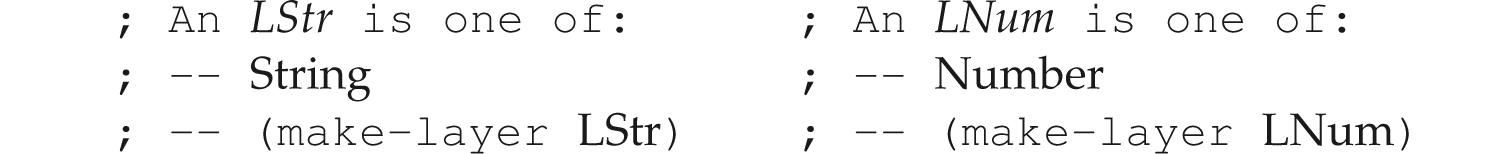
\includegraphics[width=0.85\textwidth]{images/00329.png}
\end{center}

这两个数据定义都依赖于以下结构体类型定义：

\begin{lstlisting}[language=BSL]
(define-struct layer [stuff])
\end{lstlisting}

两者都定义了嵌套形态的数据：一个是关于数字的，另一个是关于字符串的。请为两者各构造若干示例。对它们进行抽象，并展示如何通过实例化抽象定义还原出原先的两个具体定义。
\end{exercise}

\begin{exercise}{非空列表抽象}{241}
对比温度非空列表（\code{NEList-of-temperatures}）与布尔值非空列表（\code{NEList-of-Booleans}）的数据定义。然后提炼出一个通用的抽象参数化数据定义 \code{NEList-of}。
\end{exercise}

\begin{exercise}{Maybe 抽象与签名解读}{242}
以下是另一个常用的参数化数据定义：

\begin{lstlisting}[language=BSL]
; A [Maybe X] is one of:
; -- #false
; -- X
\end{lstlisting}

请解读下列数据定义的含义：\code{[Maybe String]}、\code{[Maybe [List-of String]]} 以及 \code{[List-of [Maybe String]]}。

此外，以下函数签名表达了什么含义？

\begin{center}
  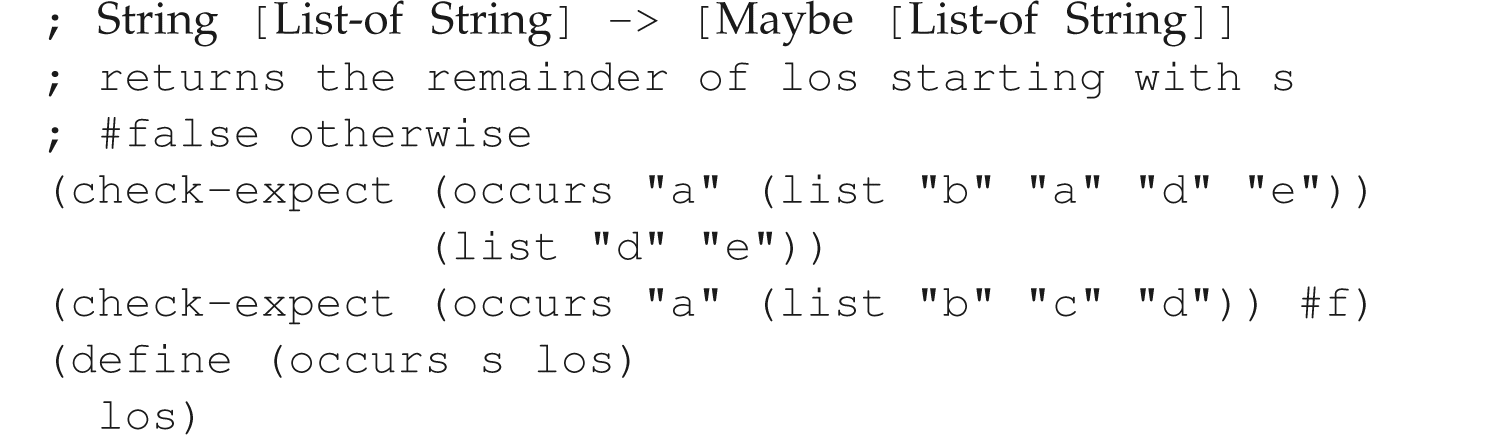
\includegraphics[width=0.85\textwidth]{images/00330.png}
\end{center}

请为其补全设计配方的其余步骤。
\end{exercise}

% ------------------------------------------------------------------------------
\section{函数即值}
\label{sec:14_4}

本部分所涉及的函数极大地拓展了我们对程序求值机制的理解。理解函数接收比数字更丰富的数据（例如字符串或图像）并不困难；结构体和列表虽然稍微复杂一些，但归根结底也是有限大小的“具体事物”。然而，\textbf{接收函数的函数}（以函数为参数的高阶函数）却显得十分奇特。事实上，这个想法在两个层面上打破了第一插曲中的语法规则：
\begin{enumerate}
  \item 原语和自定义函数的名字被作为实参传递给函数调用；
  \item 形参直接出现在函数调用表达式的首项（即函数名所在的位置）。
\end{enumerate}

明确了这个问题，就能看出 ISL 的语法与 BSL 究竟有何不同。首先，表达式语言必须允许函数名和内置原语名称像普通变量一样出现在参数位置。其次，在函数调用表达式的首项，除了固定的函数名和原语操作之外，必须允许出现形参和局部变量。

语法的这一放宽似乎要求对求值规则做出彻底变革，但实际上，我们只需要对\term{值的集合}（set of values）进行拓展：为了支持函数作为其他函数的参数，最根本的改变就是明确宣布：\term{函数与原语操作本身就是一等公民的值}（values）。

\begin{exercise}{辨识函数值}{243}
假设 DrRacket 的定义区中包含：

\begin{lstlisting}[language=BSL]
(define (f x) x)
\end{lstlisting}

判断以下表达式中哪些是\textbf{值}（values）：
\begin{enumerate}
  \item \code{(cons f '())}
  \item \code{(f f)}
  \item \code{(cons f (cons 10 (cons (f 10) '())))}
\end{enumerate}
请详细解释它们为什么是值，或者为什么不是值。
\end{exercise}

\begin{exercise}{合法表达式与文法放宽}{244}
论证为什么以下函数定义在 ISL 中是完全合法的：
\begin{enumerate}
  \item \code{(define (f x) (x 10))}
  \item \code{(define (f x) (x f))}
  \item \code{(define (f x y) (x 'a y 'b))}
\end{enumerate}
请给出你的推导与推理过程。
\end{exercise}

\begin{exercise}{函数相等性判断}{245}
开发一个名为 \code{function=at-1.2-3-and-5.775?} 的函数。给定两个从数字到数字的函数，该函数判断这两个函数在输入分别为 1.2、3 和 -5.775 时是否产生相同的结果。

数学家认为，如果两个函数在给定相同输入时总是计算出相同的结果——对于所有可能的输入皆如此——那么这两个函数就是相等的。

我们能否期望定义一个通用的 \code{function=?}，用于判定任意两个从数字到数字的函数是否在数学上严格相等？如果可以，请定义该函数；如果不可以，请解释原因，并思考这背后的深刻寓意：你遇到了第一个能够轻松用自然语言表述、却无法编写程序来判定的问题（不可判定性）。
\end{exercise}

% ------------------------------------------------------------------------------
\section{函数的求值计算}
\label{sec:14_5}

从 BSL+ 到 ISL 的转变，允许了将函数作为实参传递，并允许在函数调用表达式的首项使用变量名。DrRacket 处理这些位置上的名字与其他地方完全一样，只不过自然地期望其求值结果是一个函数。令人惊喜的是，代数中的经典\term{代换法则}（laws of substitution）稍作调整，就足以对 ISL 程序进行严格精确的求值推导。

让我们看看第 14.2 节中的 \code{extract} 函数是如何工作的。显而易见，以下等式成立：

\begin{lstlisting}[language=BSL]
(extract < '() 5) == '()
\end{lstlisting}

我们可以运用插曲 1 中的代换法则，继续在函数体内进行计算。与以往一样，形参 \code{R}、\code{l} 和 \code{t} 分别被实参 \code{<}、\code{'()} 和 \code{5} 代换。从这里开始，完全是朴素的算术与条件分支求值：

\begin{center}
  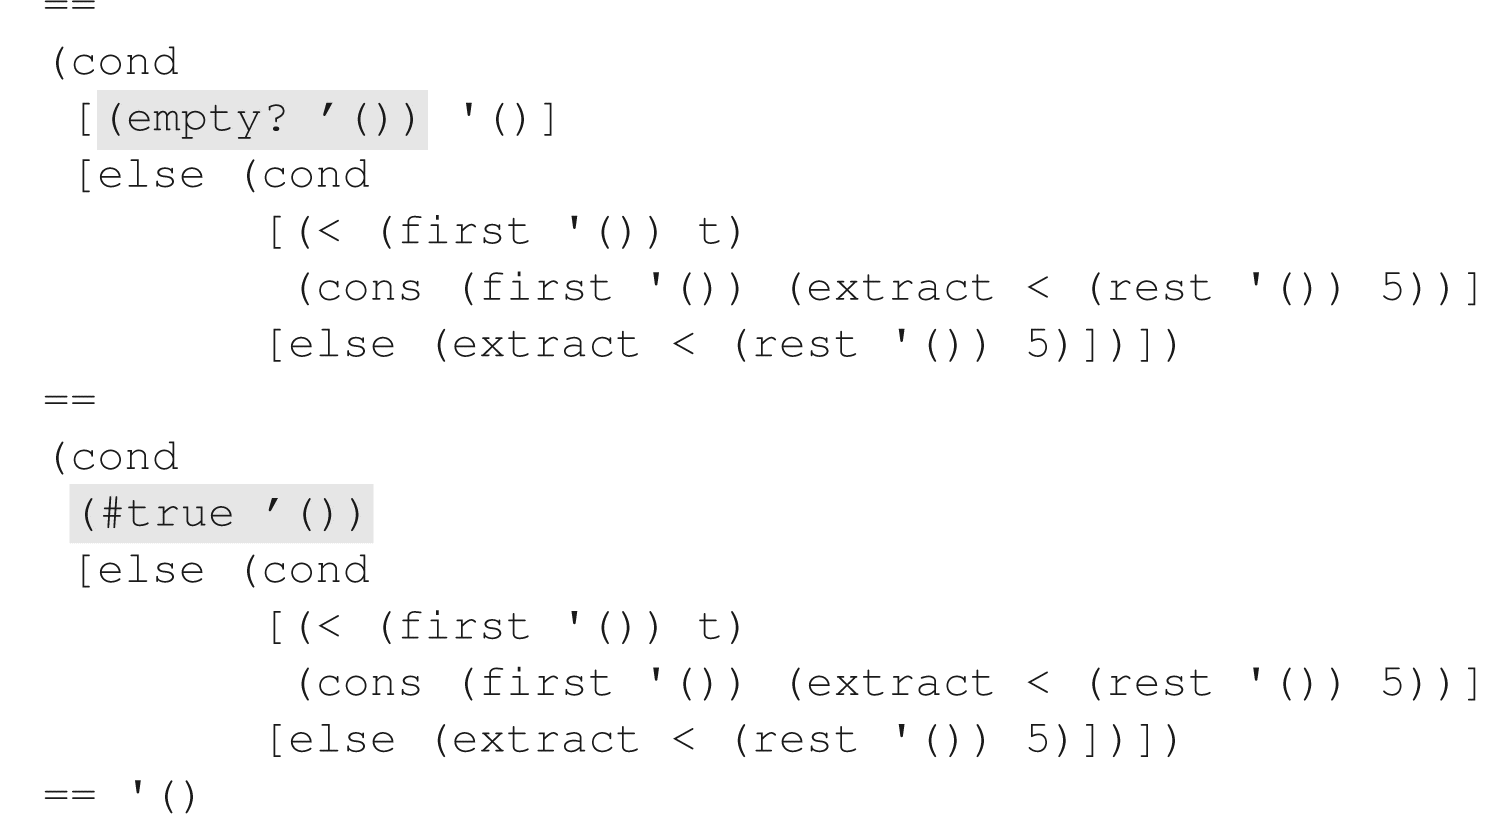
\includegraphics[width=0.85\textwidth]{images/00331.png}
\end{center}

接下来我们看一个包含单元素的列表：

\begin{lstlisting}[language=BSL]
(extract < (cons 4 '()) 5)
\end{lstlisting}

其结果应该是 \code{(cons 4 '())}，因为列表中唯一的元素是 4，且 \code{(< 4 5)} 为真。以下是单步求值的第一步：

\begin{center}
  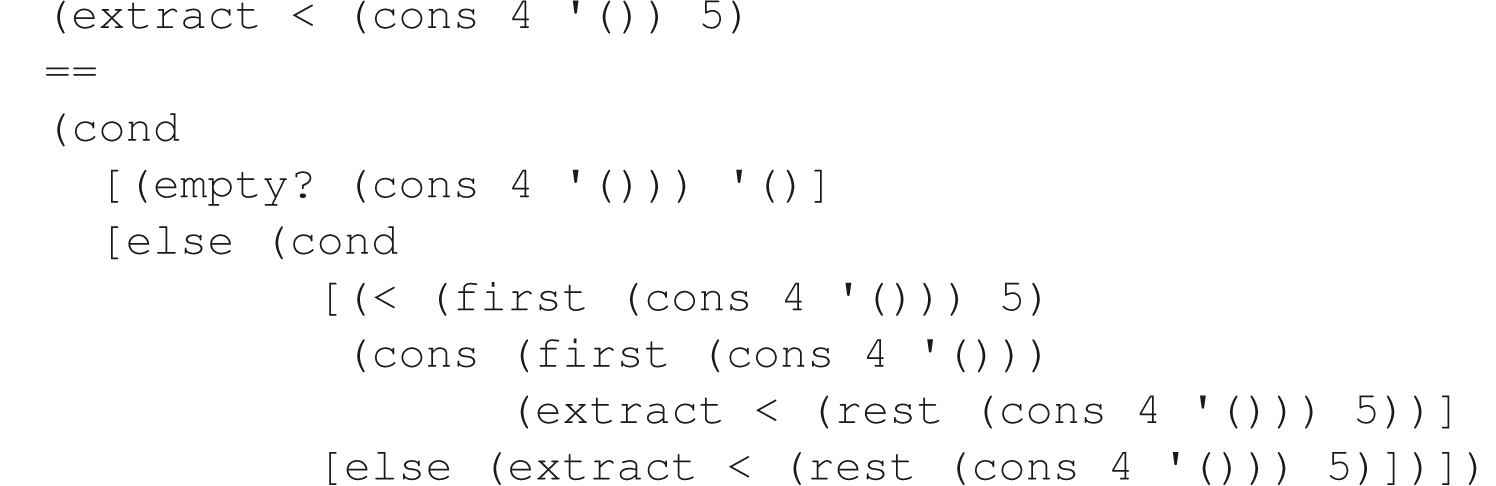
\includegraphics[width=0.85\textwidth]{images/00332.png}
\end{center}

同样，所有出现的 \code{R} 都被替换为 \code{<}，\code{l} 被替换为 \code{(cons 4 '())}，\code{t} 被替换为 \code{5}。接下来的计算直截了当：

\begin{center}
  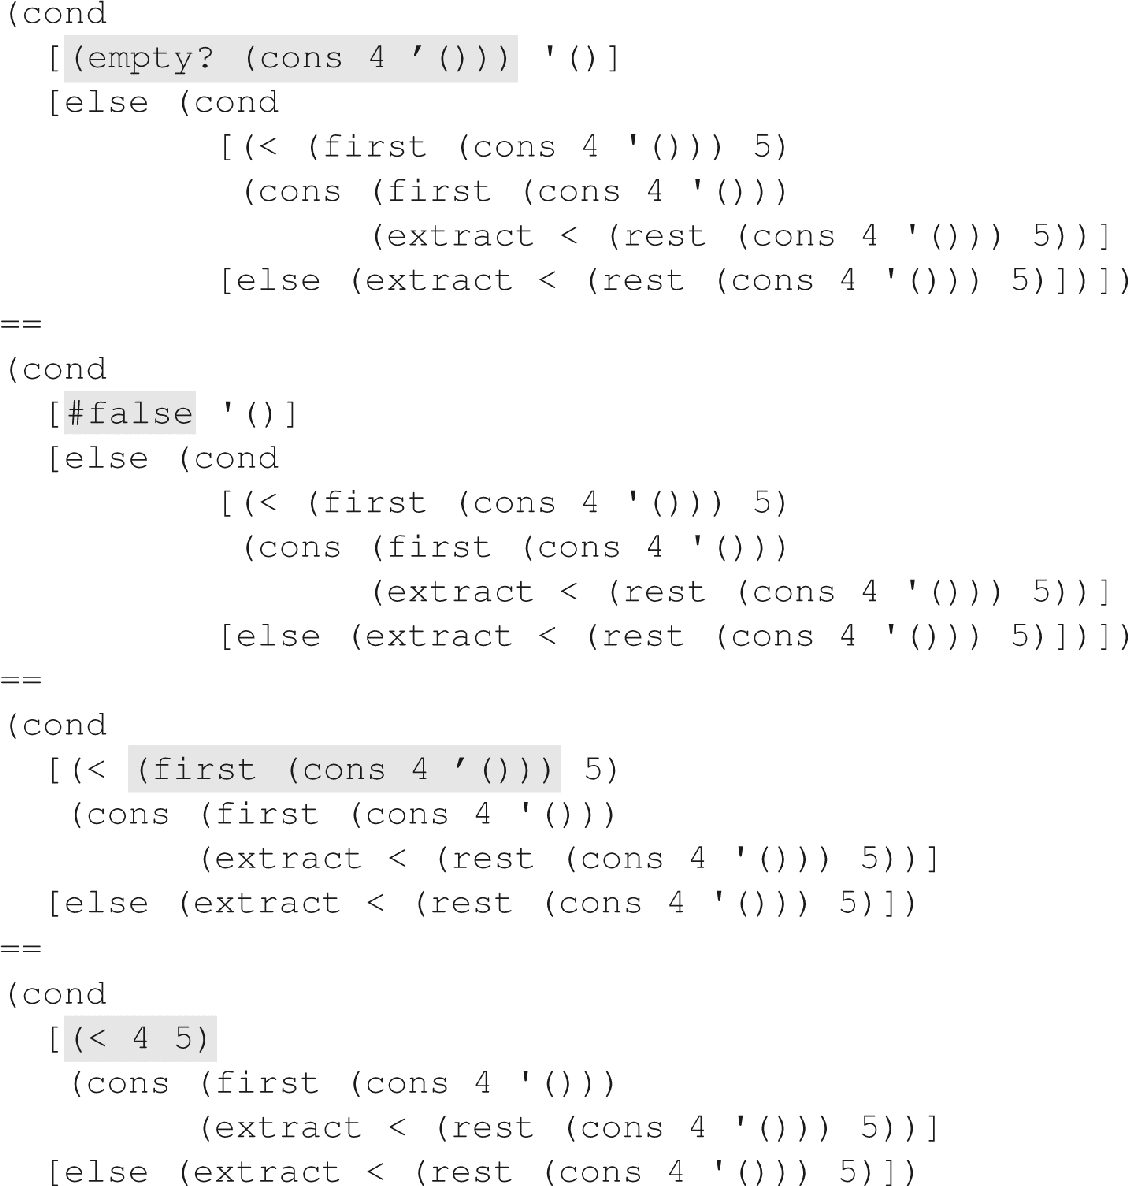
\includegraphics[width=0.85\textwidth]{images/00333.png}
\end{center}

这是最关键的一步：\code{<} 在被代换到函数调用首位后，作为普通的比较函数被直接应用。随后继续进行算术化简：

\begin{center}
  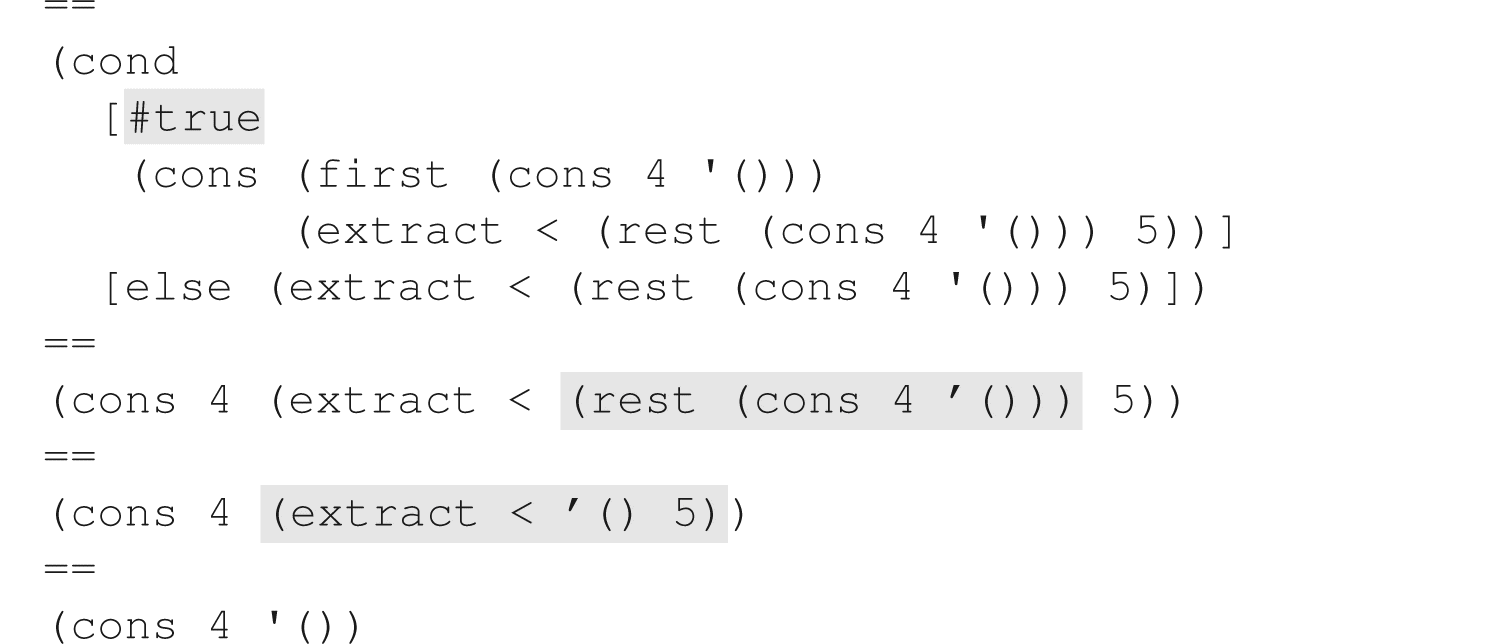
\includegraphics[width=0.85\textwidth]{images/00334.png}
\end{center}

最后一步正是上面已经证明过的等式，这意味着我们可以直接应用“等量代换”的代数公理。

我们的最后一个示例是将 \code{extract} 应用于一个包含两个元素的列表：

\begin{center}
  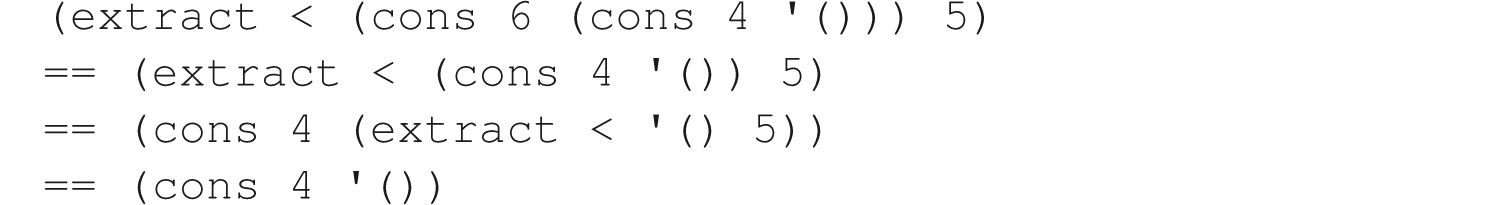
\includegraphics[width=0.85\textwidth]{images/00335.png}
\end{center}

其中的步骤 1 是全新的情形，它处理了当列表首项不小于阈值时，\code{extract} 如何将其剔除的情况。

\begin{exercise}{验证单步求值}{246}
使用 DrRacket 的单步求值器（Stepper），单步检验上一计算过程中的步骤 1：

\begin{center}
  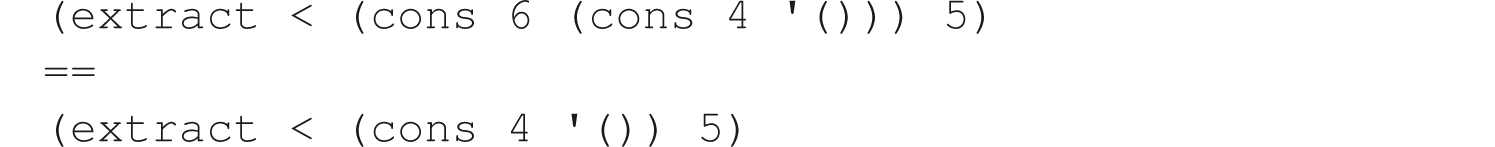
\includegraphics[width=0.85\textwidth]{images/00336.png}
\end{center}
\end{exercise}

\begin{exercise}{单步求值器跟踪 extract}{247}
使用 DrRacket 的单步求值器，完整跟踪并观察 \code{(extract < (cons 8 (cons 4 '())) 5)} 的求值全过程。
\end{exercise}

\begin{exercise}{高阶谓词的单步跟踪}{248}
在 DrRacket 单步求值器中跟踪求值 \code{(squared>? 3 10)} 和 \code{(squared>? 4 10)}。

请看以下交互会话：
\begin{replbox}
> (extract squared>? (list 3 4 5) 10)
(list 4 5)
\end{replbox}

以下是单步求值器展示的部分关键步骤：

\begin{center}
  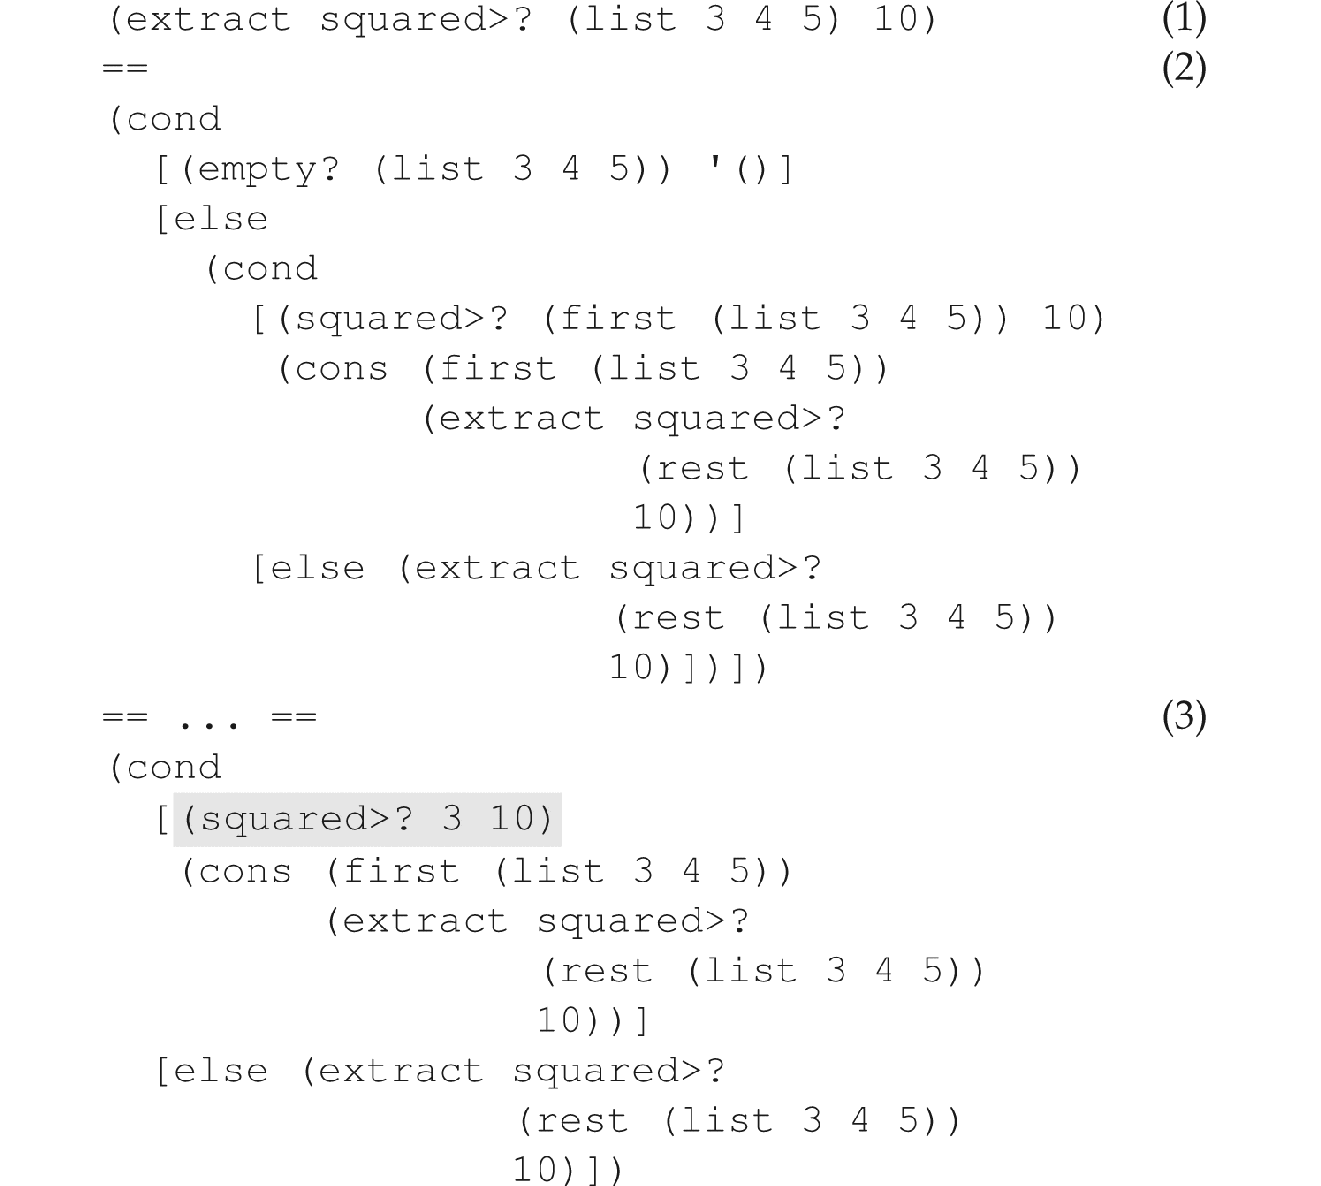
\includegraphics[width=0.85\textwidth]{images/00337.png}
\end{center}

使用单步求值器确认从第 (1) 步到第 (2) 步的推导。继续步进以填补第 (2) 步和第 (3) 步之间的细节空白。将每一步推导解释为代数法则的具体应用。
\end{exercise}

\begin{exercise}{作为值的函数求值过程}{249}
函数即值：可以作为实参、作为返回值、作为列表中的元素。将以下定义和表达式放置在 DrRacket 的定义窗口中，并使用单步求值器探究该程序的求值机制：

\begin{lstlisting}[language=BSL]
(define (f x) x)
(cons f '())
(f f)
(cons f (cons 10 (cons (f 10) '())))
\end{lstlisting}

单步求值器会将函数显示为 \code{lambda} 表达式；详见第 17 章。
\end{exercise}
